\documentclass[UTF8]{ctexart}
\usepackage{graphicx}
\graphicspath{{img/}} 
\title{Homework\ 1}
\author{PB17111623}
\author{PB17111623 范睿}
\date{\today}
\usepackage[a4paper,bottom=3.5cm]{geometry}
\usepackage{algorithm}  
\usepackage{algorithmicx}
\usepackage{amsmath}  
\usepackage{algpseudocode}  %算法的包
\usepackage{amssymb}
\begin{document}
\maketitle
\section{HW1}
\subsection{2.1-1}
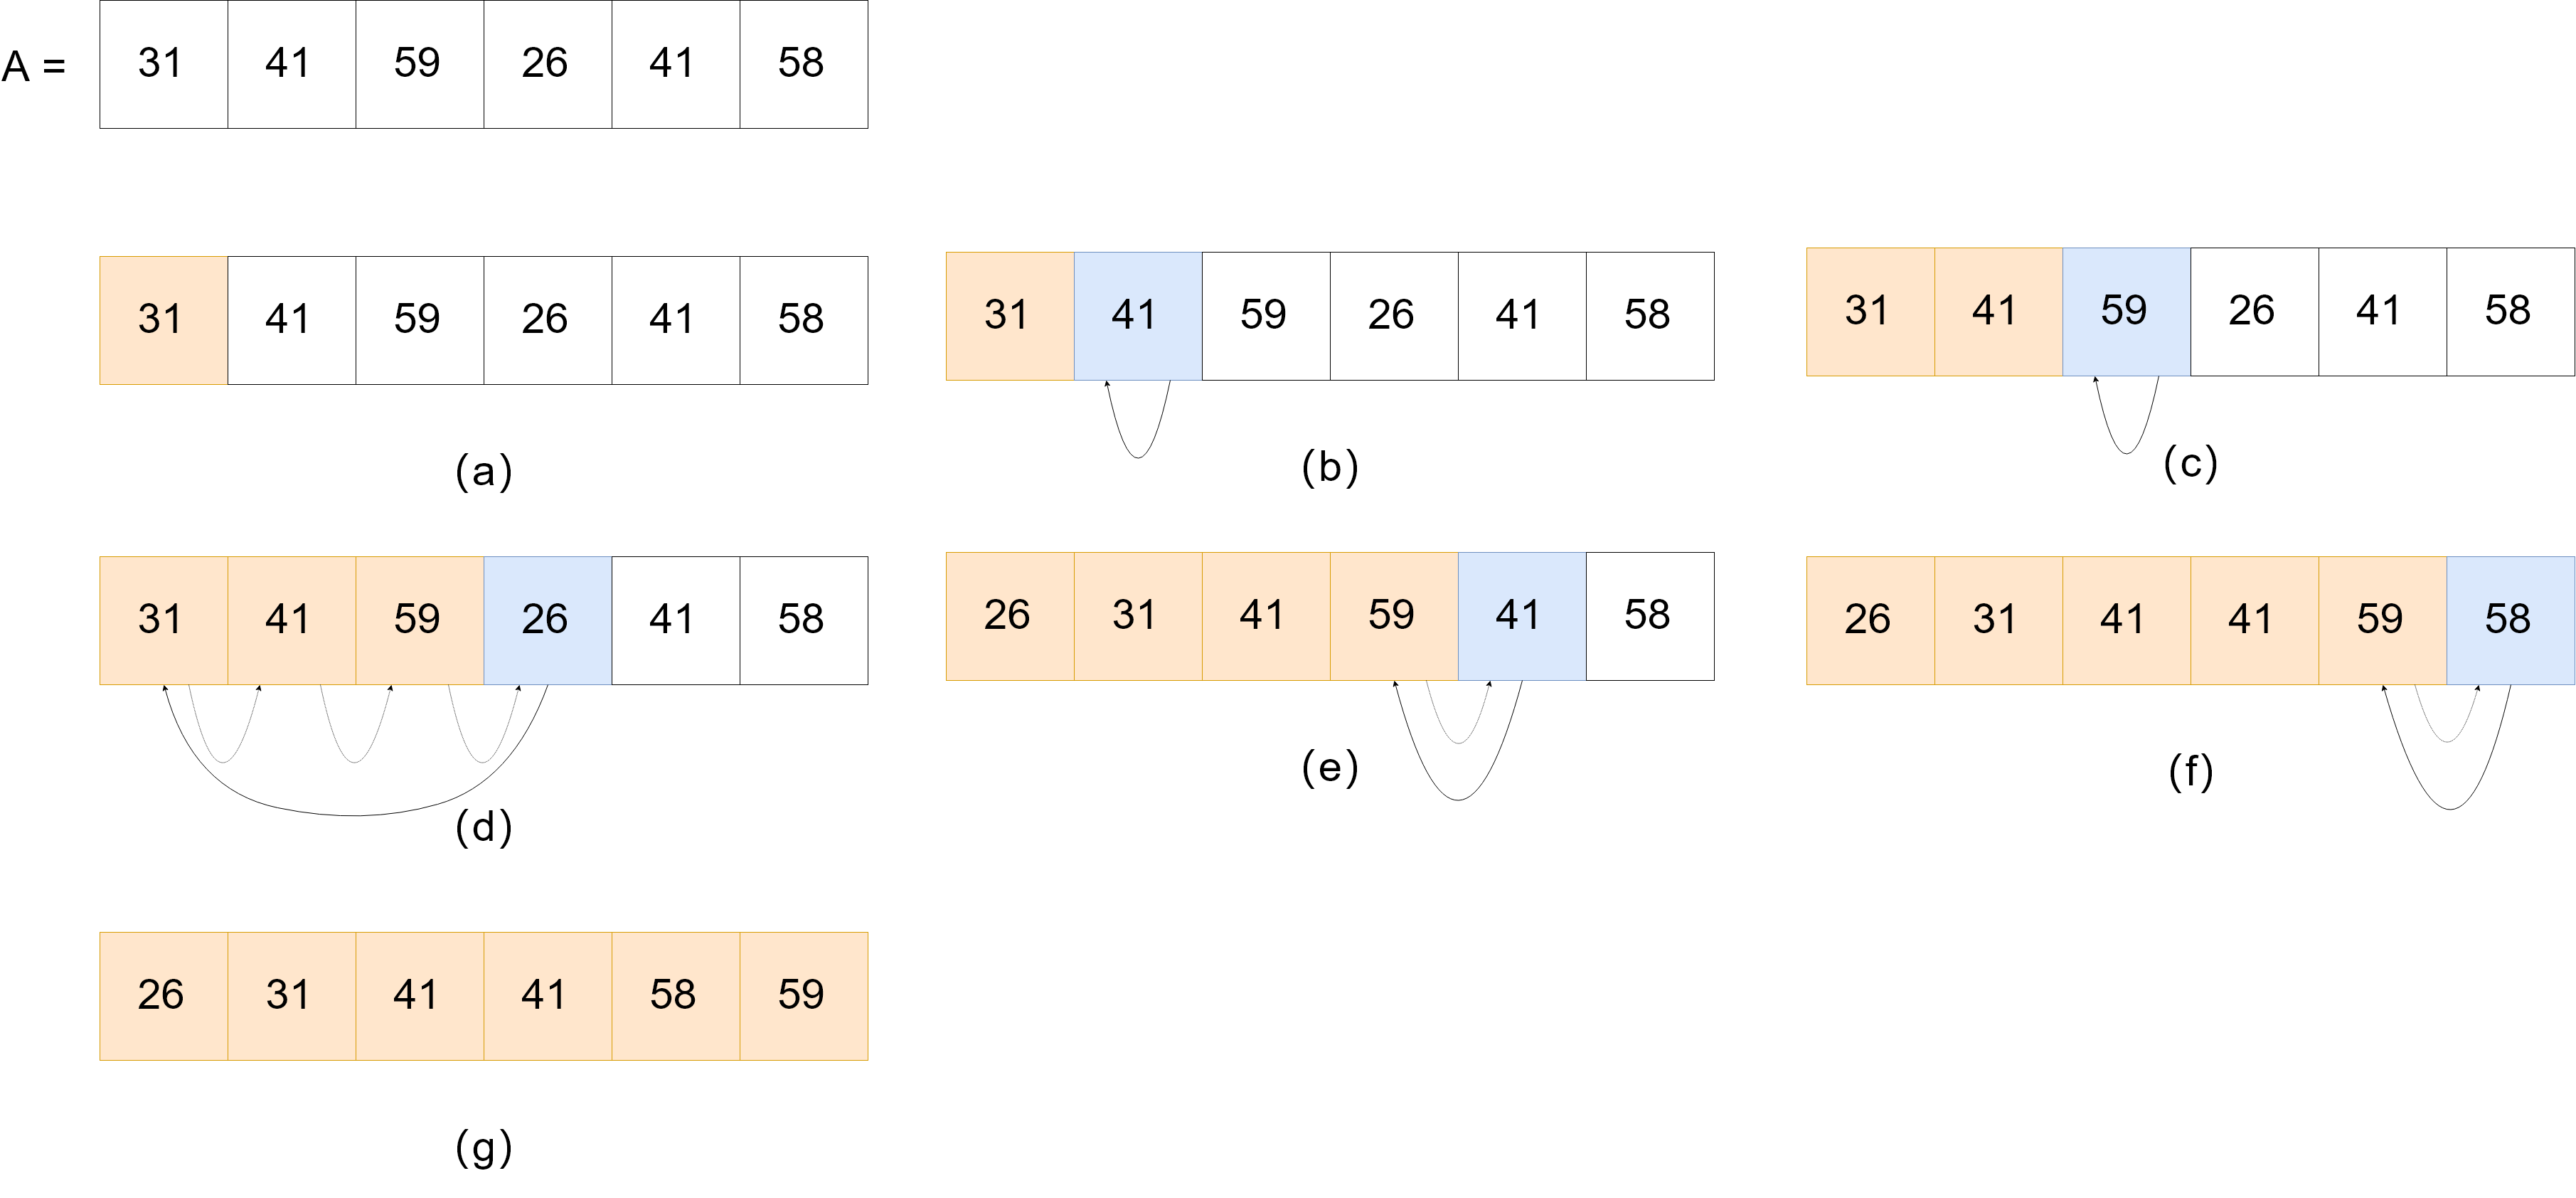
\includegraphics[scale=0.1]{21-1.png}
\paragraph{最开始,数组A没有被排序。(图中最上方,背景为全白色,代表全部未排序)}
\paragraph{(a)给前一个元素排序,因为只有一个元素,所以直接是排好序的(背景为黄色)}
\paragraph{(b)给前两个元素排序,41比31大,不交换}
\paragraph{(c)给前三个元素排序,59比41大,不交换}
\paragraph{(d)给前四个元素排序,26比31小,发生三次交换,将26排到数组最前方}
\paragraph{(e)给前五个元素排序,41比59小,和41一样,发生一次交换,将41移至第四个位置}
\paragraph{(f)给前六个元素排序,58比59小,比41大,发生一次交换,将58移至第五个位置}
\paragraph{(g)此时全部元素已排好顺序}
\subsection{2.1-3}
\floatname{algorithm}{算法}
\renewcommand{\algorithmicrequire}{\textbf{输入:}}
\renewcommand{\algorithmicensure}{\textbf{输出:}}
\begin{algorithm}
	\caption{线性查找}
	\begin{algorithmic}[1]%显示行号
	\Require 序列$A=<a_1, a_2, ..., a_n>$, 值$v$
	\Ensure 下标$i$使得$A[i]=v$或者$v$不在$A$中出现时,输出$NIL$
	\For{$i = 0\to A.length-1$}
		\If{$A[i]\ =\ v$}
			\State \Return{$i$}
		\EndIf
	\EndFor
	\State \Return{$NIL$}
	\end{algorithmic}
\end{algorithm}
\paragraph{证明:\\}
取循环不变式为:\\\emph{ \qquad每一次for循环开始前,数组A的前i个位置的元素都没有和v相同的元素}\\
\textbf{初始化:\\}第一次循环开始前,i=0,满足A数组前0个元素没有和v相同的元素,满足。
\textbf{\\保持:\\}假设第k次循环开始前,数组A前k-1个位置的元素没有和v相同的,那么在第k次循环中,若A[k-1]=v,程序将返回,不会到达下一次循环。所以如果可以到达第k+1第循环,则说明A[k-1]与v不相同。又因为前k-1个元素与v均不同为假设,可以推出在第k+1循环开始前,A数组中前k个元素与v均不相同。
\textbf{\\终止:\\}for循环有两个终止条件:①i=A.length-1②A[i]=v\\
①i=A.length-1:此条件满足时,说明A数组的前A.length个元素均不与v相同,即A中所有元素均不与v相同,此情况下,算法返回NIL,满足题目要求\\
②A[i]=v:此条件满足时,算法找到了A中的一个与v相同的元素,它的下标即为i。此情况下,算法返回下标i,满足题目要求。\\
综上,算法正确。

\subsection{2.2-3}
平均输入:$\frac{n+1}{2}$\\
最坏输入:n\\
平均查找时间:{$\Theta(n)$}\\
最坏查找时间:{$\Theta(n)$}\\
证明:\\
①证明平均查找时间\\
存在$c_1=\frac{1}{2}\quad c_2=1$,使得当n足够大时,$c_1n \leq n \leq c_2n$恒成立\\
②证明最坏查找时间\\
存在$c_1=1\quad c_2=1$,使得当n足够大时,$c_1n \leq n \leq c_2n$恒成立

\end{document}
